\begin{graphicspathcontext}{{./chapters/mas/examples/imgs/auto/},\old}

\sidenote{\cite{Ferber.1999}, Image Clause Sonet 4.6}
\begin{frame}[t]{Forager Bots}
	\begin{block}{Scenario \cite{Ferber.1999}}
		\smaller A colony of \emph{autonomous robots} (bots) operates in a shared environment.
		Their collective goal is to \emph{gather food items} scattered across the environment and bring them back to a central \emph{nest (base camp)}
	\end{block}
	\begin{columns}
		\begin{column}{.5\linewidth}
			\begin{block}{Key Elements}
				\begin{description}
					\item[Agents] forager bots
					\item[Environment] a 2-D grid or continuous space
					\item[Resources] food items spread randomly
					\item[Base] nest where food is deposited
				\end{description}
			\end{block}
		\end{column}
		\begin{column}{.5\linewidth}
			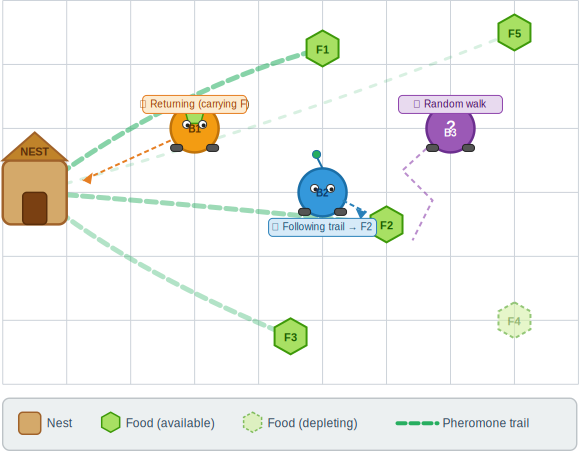
\includegraphics{forager_bots}
		\end{column}
	\end{columns}
\end{frame}

\begin{frame}[fragile]{Forager Agent Loop}
	\begin{columns}
		\begin{column}{.5\linewidth}
				\begin{sarllisting}
def run() {
	var done = false
	while (!done) {
	  var p = get_percept()
	  var a = choose_action(p)
	  do_action(a)
	  done = check_if_done()
	}
	die()
}\end{sarllisting}
		\end{column}
		\begin{column}{.5\linewidth}
			\smaller
			\begin{block}{\texttt{get\_percept()}}
				\begin{compactdescription}
				\item[Sense nearby cells] food present? pheromone level? other bots?
				\item[Read internal state] \emph{carrying food?} current position
				\end{compactdescription}
			\end{block}
			\begin{block}{\texttt{do\_action()}}
				\begin{compactdescription}
				\item[Move] to an adjacent cell (towards food or towards nest)
				\item[Pick up] a food item (if on a food cell and not loaded)
				\item[Drop] food at the nest (if carrying and at nest)
				\item[Deposit pheromone] on the current cell
				\item[Update internal state] toggle \texttt{carrying\_food} flag; update position
				\end{compactdescription}
			\end{block}
		\end{column}
	\end{columns}
\end{frame}

\begin{frame}{Forager Decision Process}
	\begin{columns}
		\begin{column}{.5\linewidth}
			\begin{block}{Mode 1 --- Foraging}
				\Emph{Constraint:} Bot is \emph{not} carrying food \\
				\Emph{Goal:} find a food item \\
				\Emph{Strategy:}
				\begin{itemize}
				\item If food is visible $\Rightarrow$ move to food \& pick it up
				\item Else if pheromone trail nearby $\Rightarrow$ follow trail
				\item Else $\Rightarrow$ random walk (exploration)
				\end{itemize}
			\end{block}
		\end{column}
		\begin{column}{.5\linewidth}
			\begin{block}{Mode 2 --- Returning}
				\Emph{Constraint:} Bot \emph{is} carrying food \\
				\Emph{Goal:} bring food to the nest \\
				\Emph{Strategy:}
				\begin{itemize}
				\item Navigate back towards the nest (gradient / memory)
				\item Deposit pheromone on the path (positive feedback)
				\item Drop food when reaching the nest
				\end{itemize}
			\end{block}
		\end{column}
	\end{columns}
\end{frame}

\sidenote{Image by Claude Sonnet 4.6}
\figureslide{Forager Flow Chart}{forager_bots_flowchart}

\begin{frame}{Emergent Behaviour}
	\begin{block}{Stigmergy}
	Bots communicate \Emph{indirectly} through the environment via pheromone
	trails.  No bot has global knowledge; yet the colony collectively discovers
	and exploits food sources efficiently.
	\end{block}
	\bigskip
	\Emph{Emergent properties observed:}
	\begin{description}
	\item Shortest paths to food are reinforced (pheromone accumulates faster)
	\item Exhausted food sources are naturally abandoned (trail evaporates)
	\item The system is \Emph{robust}: losing one bot does not break the colony
	\item[Scalability] adding more bots increases throughput without redesigning any individual agent.
	\end{description}
\end{frame}

\end{graphicspathcontext}

\endinput

